\documentclass[10pt,twocolumn,a4paper]{article}

\usepackage[portuguese]{babel}
\usepackage[utf8]{inputenc}
\usepackage[margin=1.5cm]{geometry}
\usepackage{graphicx}
\usepackage{amsmath}
\usepackage{hyperref}
\usepackage{caption}
\usepackage{subcaption}
\usepackage{authblk}

\title{\textbf{Busca Semântica no Contexto de Desinformação Vacinal}\\[0.3cm]
\large MO850 - Tópicos Avançados em Ciência da Computação\\[0.1cm]Instituto de Computação (IC) - Unicamp}
\author{Daniele Souza Gonçalves\\ RA: 248029 \\ \texttt{d248029@dac.unicamp.br}}
\date{}

\frenchspacing

\begin{document}
\maketitle

\begin{abstract}
Este relatório descreve a aplicação de técnicas de Processamento de Linguagem Natural e busca semântica utilizando embeddings contextuais (SBERT) para a análise de narrativas de desinformação no dataset Aletheia. Foi aplicada a modelagem de tópicos com BERTopic para extrair clusters não-supervisionados e correlacionar os padrões semânticos e temporais com as narrativas de desinformação vacinal que circulam nas redes sociais, visando superar a limitação da busca léxica tradicional.
\end{abstract}

\section{Introdução e Motivação}

Este trabalho trata do uso de busca semântica no contexto da desinformação vacinal. Sabe-se que as redes sociais, como o Telegram, sofrem com uma propagação frequente de notícias contendo desinformação e \textit{fake news}, e no cenário da hesitação vacinal isso não é diferente. Esse tipo de conteúdo tem o potencial de gerar crises de saúde pública agudas, como as testemunhadas no Brasil durante a pandemia de COVID-19.

Métodos de busca tradicionais, como a busca léxica simples por palavras-chave, frequentemente falham em capturar as complexidades e sutilezas dessas campanhas de desinformação, uma vez que elas fazem uso intensivo de eufemismos, abreviações, ironia ou linguagem conspiratória e codificada. Essa limitação é a principal motivação deste trabalho para utilizar a \textbf{busca semântica}, já que os embeddings contextuais capturam as relações de significado de maneira muito superior às correspondências literais de tokens.

Portanto, este projeto busca responder a três questões centrais de pesquisa:
\begin{enumerate}
    \item A busca semântica via embeddings contextuais consegue recuperar narrativas de desinformação de forma mais abrangente que a busca léxica?
    \item Os modelos de linguagem (LLMs), em configuração \textit{zero-shot}, são confiáveis para classificar e validar mensagens de desinformação quando comparados à anotação humana?
    \item Quais são os padrões temáticos, de volume, de evolução temporal e de engajamento público que emergem do discurso antivacina nestes canais?
\end{enumerate}

Todos os códigos, análises e cadernos interativos desenvolvidos para este projeto estão disponíveis publicamente no repositório do GitHub e podem ser acessados em: \url{https://github.com/danielegsouza/MO850-final-project}.

\section{Metodologia}

\subsection{Processamento e Filtragem}
O conjunto de dados original estudado baseia-se no \textit{Brazilian Social Media Anti-vaccine Information Disorder Dataset} (Aletheia \cite{aletheia_unicamp}). Oficialmente, este dataset abriga quase 4 milhões de postagens do Telegram, coletadas de 119 proeminentes canais e grupos antivacina brasileiros entre janeiro de 2020 e junho de 2025. Para viabilizar os experimentos deste projeto, foi utilizada uma amostra estruturada do Aletheia \cite{aletheia_sample}, contendo cerca de $64.000$ mensagens, amostradas em $1.000$ mensagens por mês (Figura \ref{fig:temporal_dist}(a)). Foi realizada uma etapa de filtragem, mantendo apenas as mensagens no idioma português, o que representava cerca de 51\% do conteúdo total (conforme distribuição ilustrada na Figura \ref{fig:language_dist}). 

Para refinar ainda mais a qualidade semântica da modelagem, foram mantidas exclusivamente as mensagens com mais de 20 tokens, a fim de eliminar textos excessivamente curtos que continham apenas saudações comuns (como "bom dia", "boa tarde"). Como resultado do processamento, o dataset final foi reduzido de $64.000$ para aproximadamente $17.700$ mensagens, cuja nova distribuição temporal pode ser observada na Figura \ref{fig:temporal_dist}(b).

\begin{figure}[htbp]
    \centering
    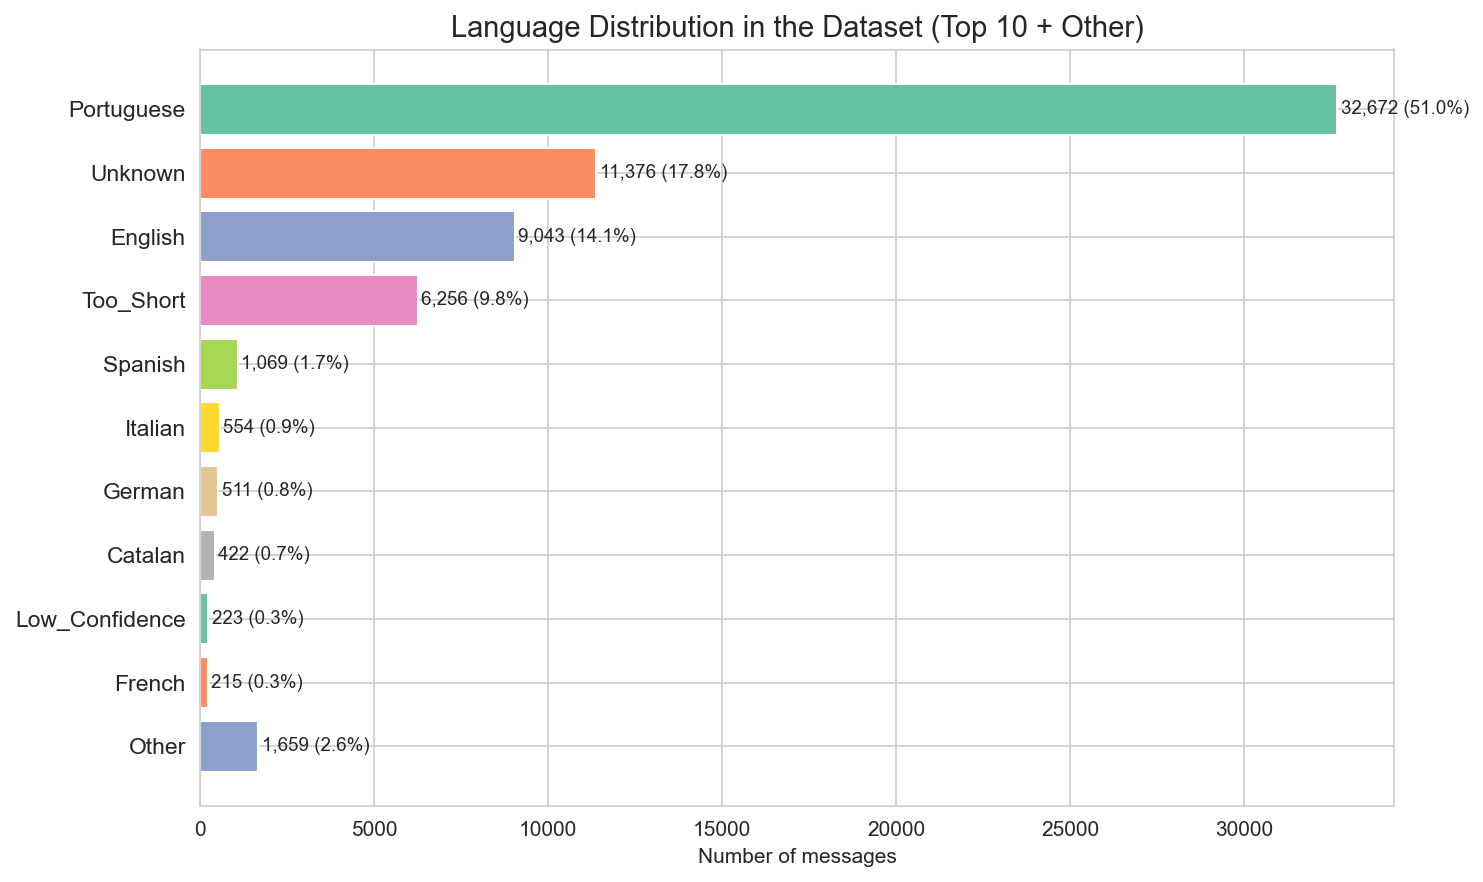
\includegraphics[width=\linewidth]{figures/01_languages.png}
    \caption{Distribuição dos idiomas identificados no corpus original.}
    \label{fig:language_dist}
\end{figure}

\begin{figure}[htbp]
    \centering
    \begin{subfigure}{\linewidth}
        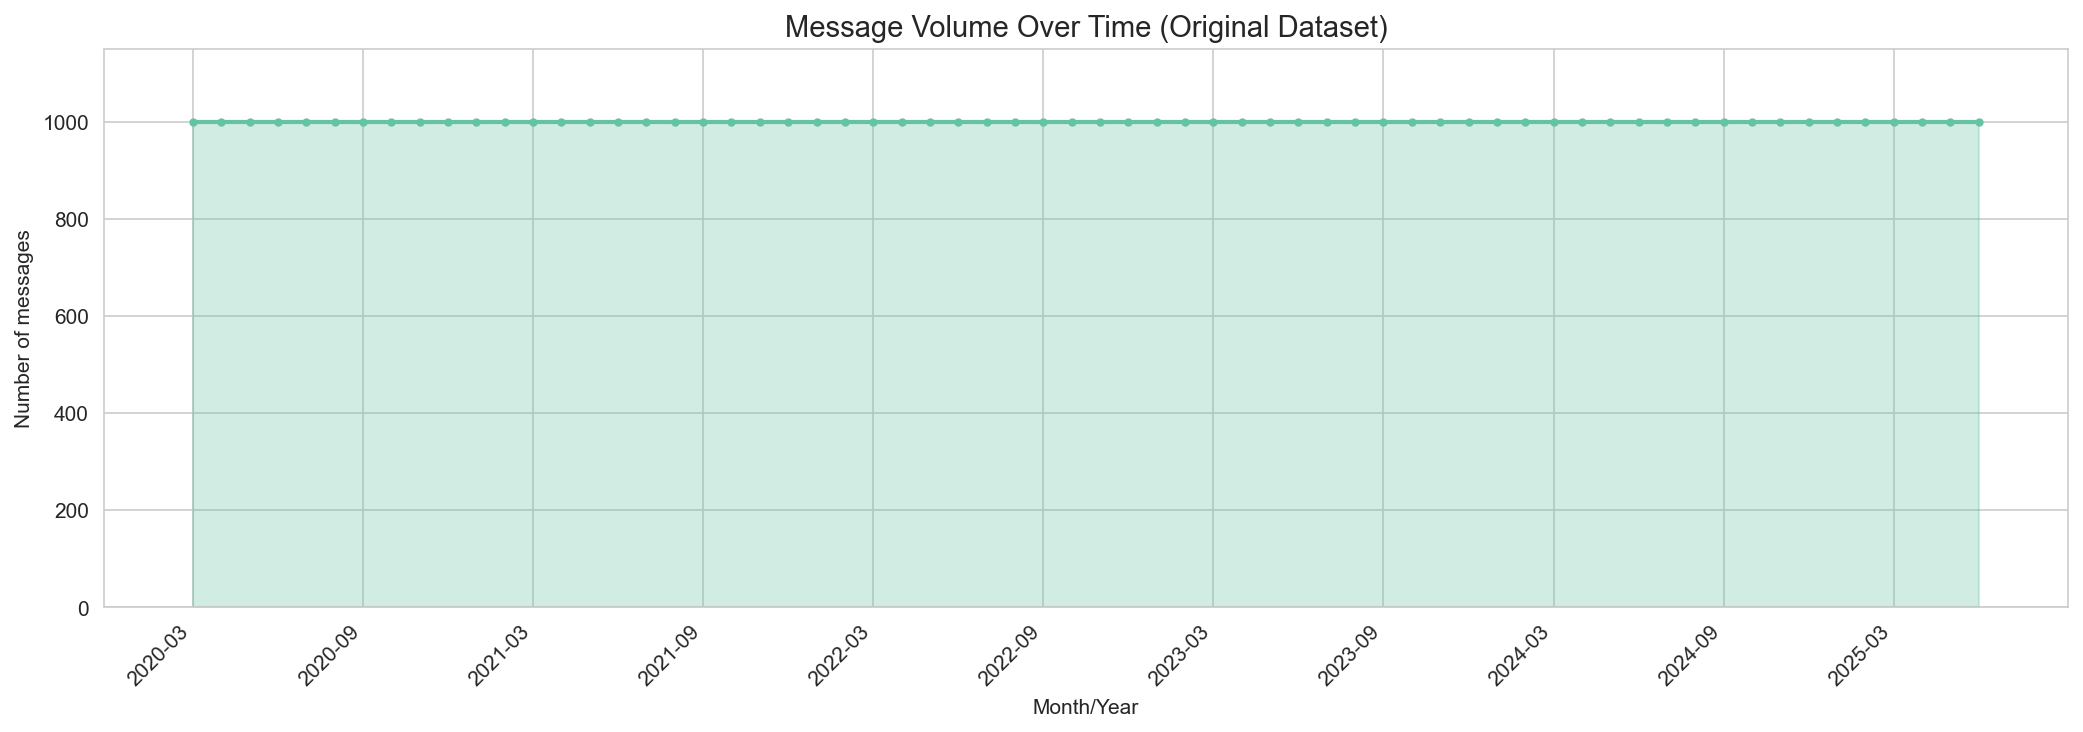
\includegraphics[width=\linewidth]{figures/01_temporal.png}
        \caption{Distribuição original ($64k$ mensagens).}
    \end{subfigure}\\
    \vspace{0.3cm}
    \begin{subfigure}{\linewidth}
        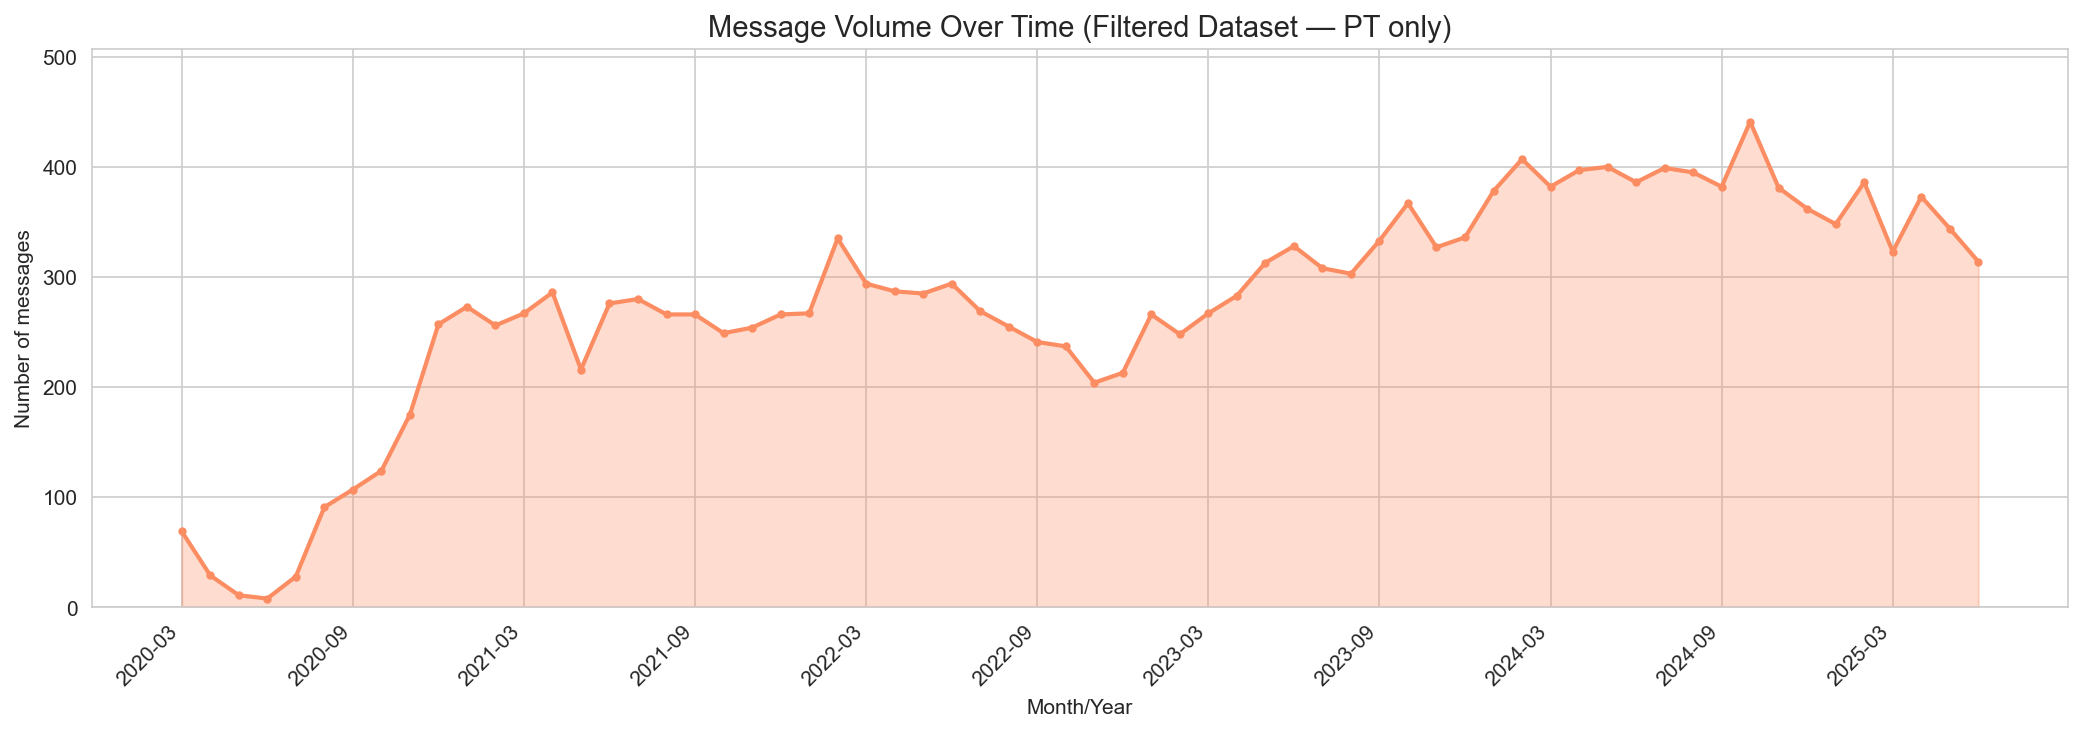
\includegraphics[width=\linewidth]{figures/01_temporal_filtered.png}
        \caption{Distribuição após filtragem ($17.7k$ mensagens).}
    \end{subfigure}
    \caption{Impacto do processamento no volume temporal do dataset.}
    \label{fig:temporal_dist}
\end{figure}

\subsection{Modelagem de Tópicos}
Para realizar a descoberta automática dos tópicos latentes no corpus, foi aplicado o algoritmo BERTopic. O fluxo interno da ferramenta foi configurado com os seguintes componentes e hiperparâmetros para adequação às características de redes sociais:

\begin{itemize}
    \item \textbf{Embeddings:} Para a geração dos vetores densos dos documentos, foi empregado o modelo SBERT multilíngue (\texttt{paraphrase\allowbreak{}-multilingual\allowbreak{}-MiniLM\allowbreak{}-L12\allowbreak{}-v2}), que produz embeddings de 384 dimensões.
    \item \textbf{UMAP:} Redução de dimensionalidade com 15 vizinhos (\textit{n\_neighbors}), 5 componentes, distância mínima de $0.0$, métrica de cosseno e \textit{random\_state} fixado em 42.
    \item \textbf{HDBSCAN:} Clusterização com tamanho mínimo de cluster igual a 30 e pelo menos 10 amostras, utilizando métrica euclidiana. Essa escolha de parâmetros (\texttt{min\_samples=10} e \texttt{min\_cluster\_size=30}) foi crucial para evitar a formação de clusters ruidosos e compostos por pouquíssimas mensagens. Considerando a natureza curta dos textos de redes sociais, esses limiares mais rígidos garantiram que os tópicos fossem minimamente coesos e representativos.
    \item \textbf{c-TF-IDF:} Antes da extração dos termos mais representativos por cluster, foi aplicada a remoção de \textit{stopwords} em português para evitar que os tópicos fossem dominados por conectivos ou palavras irrelevantes.
\end{itemize}

\section{Resultados e Análise}

\subsection{Descoberta de Tópicos e Tratamento de Ruído}
Com as configurações estabelecidas, o algoritmo identificou um total de \textbf{78 tópicos distintos}. Um ponto de atenção é que o tópico \texttt{-1} (que representa os \textit{outliers} ou ruído não clusterizado pelo HDBSCAN) representou 47.2\% do dataset, o equivalente a $8.363$ mensagens.

Embora pareça elevado, esse percentual é totalmente esperado e comum na literatura quando se trata de modelagem de tópicos não supervisionada em dados de redes sociais. A natureza fragmentada, genérica e ruidosa do Telegram contém muita conversa solta, URLs e mensagens sem coesão narrativa suficiente para formar um grupo denso. O comportamento conservador do HDBSCAN, ao classificar esses pontos de baixa densidade como ruído, preservou a altíssima qualidade semântica e coerência dos 78 tópicos restantes que, de fato, interessam para a pesquisa.

\begin{figure}[htbp]
    \centering
    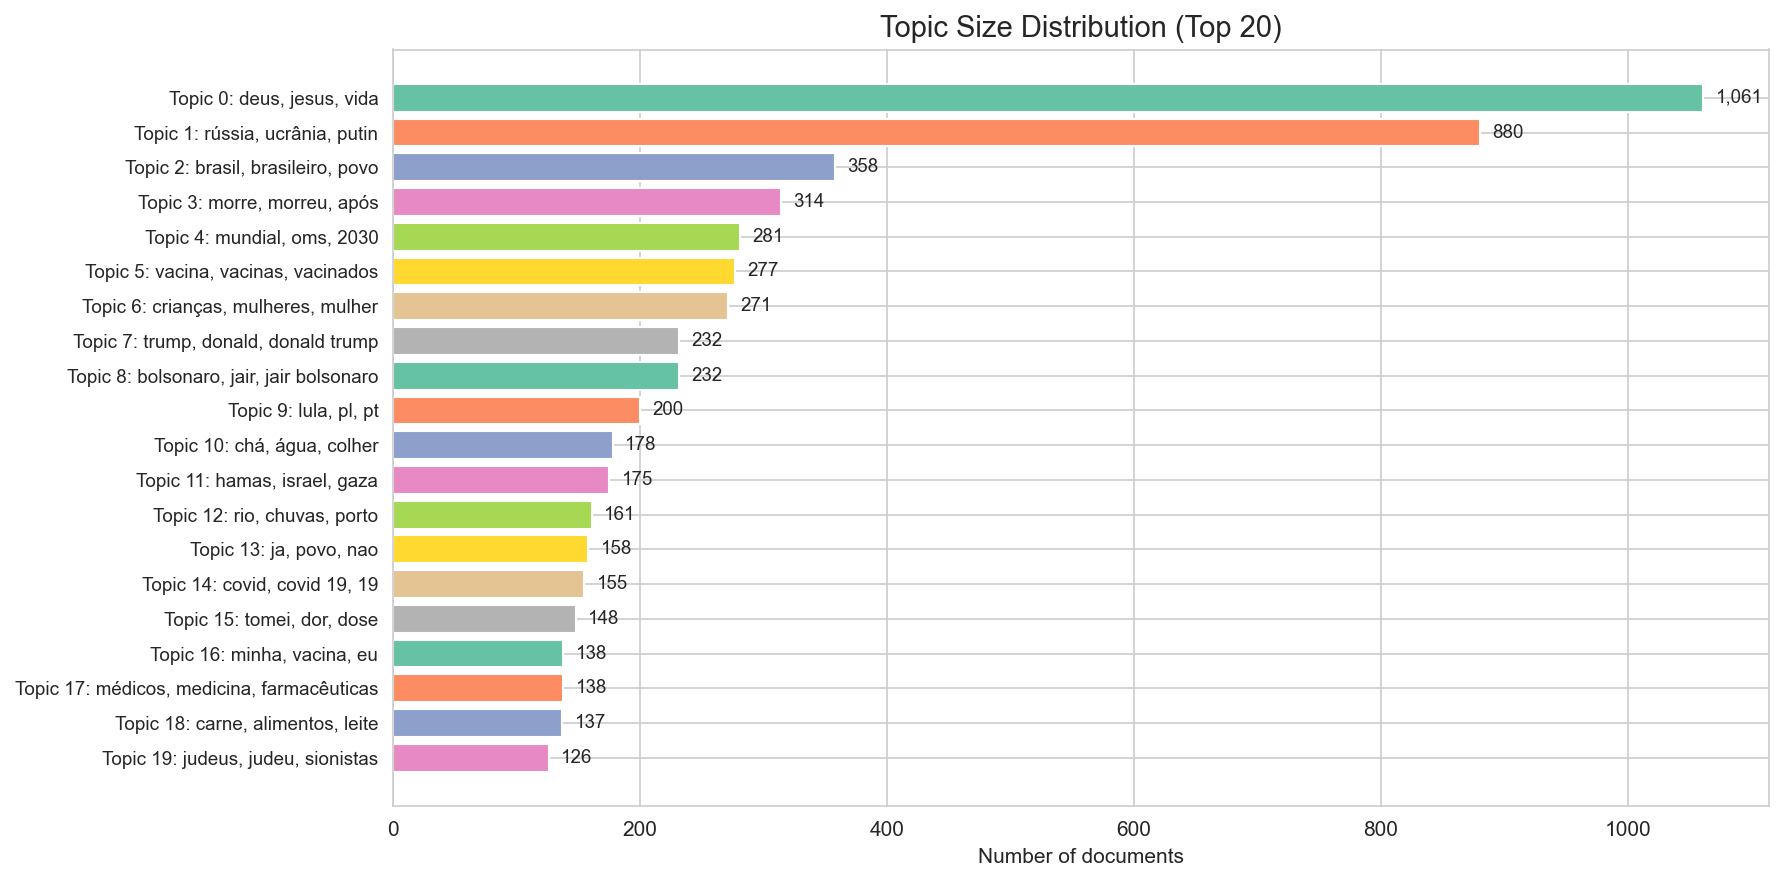
\includegraphics[width=\linewidth]{figures/02_topic_sizes.png}
    \caption{Distribuição do tamanho dos tópicos descobertos.}
    \label{fig:topic_sizes}
\end{figure}

\subsection{Eixos Temáticos do Discurso Anti\mbox{vacina}}

Avaliando os 78 clusters (Figura \ref{fig:top_terms}), foi possível observar de maneira evidente os eixos centrais do discurso anti\mbox{vacina} e as narrativas predominantes nos canais estudados.

Os maiores agrupamentos mapearam temas bastante nítidos, sendo possível destacar: \textbf{Tópico 0} (discussões sobre religião e moralidade); \textbf{Tópico 1} (a guerra entre Rússia e Ucrânia); \textbf{Tópico 2} (identidade nacional e discurso pró-Brasil); \textbf{Tópico 3} (relatos alarmistas sobre mortes e efeitos adversos das vacinas); \textbf{Tópico 4} (teorias da conspiração envolvendo organizações globais como a OMS e a ONU); e \textbf{Tópico 5} (o eixo central focado majoritariamente na própria vacinação).

Foi notada, também, a menção frequente a grupos demográficos específicos no \textbf{Tópico 6} (mulheres, pessoas trans e comunidade LGBT). Adicionalmente, a política internacional se destacou no \textbf{Tópico 7}, impulsionada por discussões sobre as eleições nos Estados Unidos e a presidência de Donald Trump.

\begin{figure*}[htbp]
    \centering
    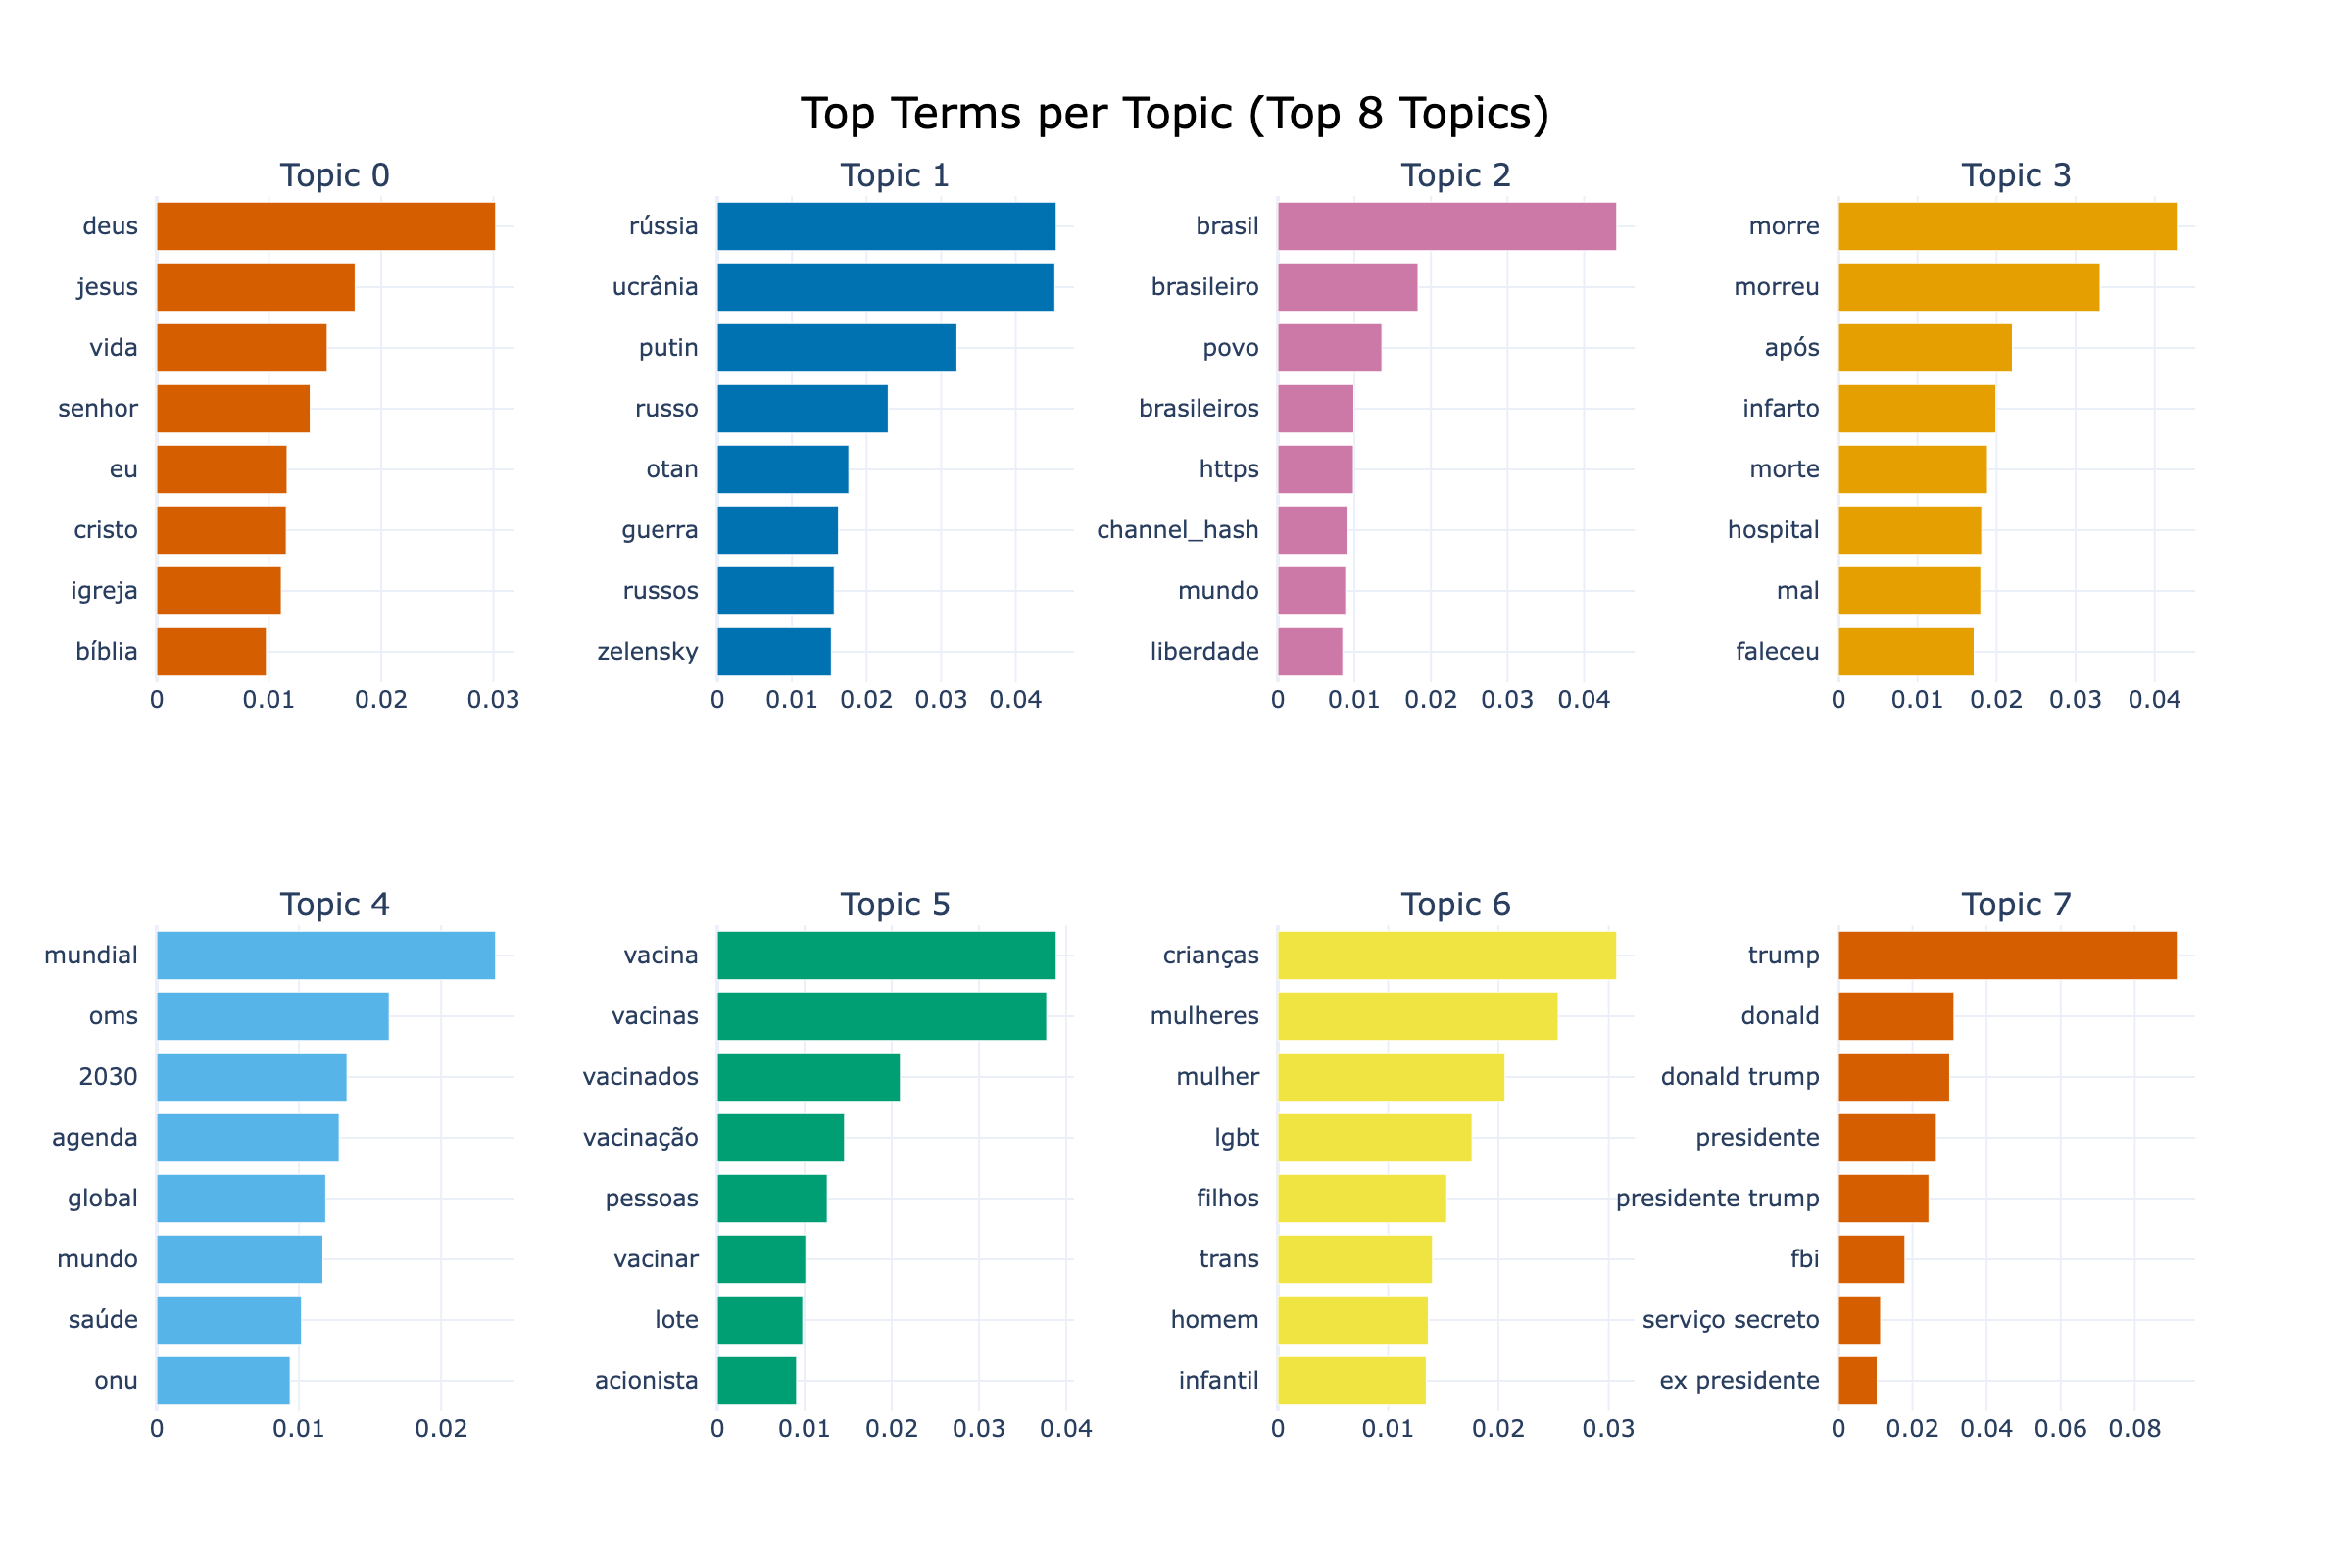
\includegraphics[width=\textwidth]{figures/02_topic_barchart.png}
    \caption{Principais termos (c-TF-IDF) extraídos para os principais tópicos descobertos.}
    \label{fig:top_terms}
\end{figure*}

\subsection{Comparação entre Busca Semântica e Léxica}

Para avaliar o desempenho na recuperação de informações, foram definidas 5 narrativas predefinidas (queries manuais) comuns em campanhas antivacina e foram executadas buscas tanto pela abordagem léxica (palavras-chave) quanto pela abordagem semântica (SBERT). 

Na busca semântica, foram recuperadas rigorosamente as 100 mensagens mais semelhantes (\textit{top-100}) para cada uma das 5 queries. É importante destacar uma diferença fundamental de comportamento entre os dois métodos: enquanto a busca léxica falha em retornar documentos caso o termo exato não seja encontrado, a busca semântica, por operar sobre distâncias vetoriais, sempre retornará um \textit{ranking} de resultados (caso haja documentos suficientes no corpus), mesmo que a similaridade seja extremamente baixa.

Cientes dessa particularidade, foram analisadas as métricas de retorno, observando-se que o menor score de similaridade retornado pela busca semântica, entre todas as $500$ mensagens recuperadas no \textit{top-100} das 5 queries, foi de \textbf{0.61}. Esse resultado é extremamente positivo, pois demonstra que, em outras palavras, a mensagem com a pior similaridade recuperada ainda mantinha um forte grau de correlação semântica com a query original, atestando a precisão do uso de embeddings para este domínio.

Para demonstrar de forma visual a cobertura e o mapeamento semântico, foram cruzados os 78 tópicos gerados pelo BERTopic com essas 5 queries narrativas. A Tabela \ref{tab:topic_mapping} detalha os dois tópicos não supervisionados com maior similaridade vetorial (\textit{Top-2}) recuperados para cada query manual. 

\begin{table*}[htbp]
    \centering
    \caption{Mapeamento Semântico: Queries Manuais vs. Tópicos Descobertos (Top-2)}
    \resizebox{\textwidth}{!}{
    \begin{tabular}{p{6cm} c c p{6cm} c}
        \hline
        \textbf{Narrativa (Query)} & \textbf{ID do Tópico} & \textbf{Similaridade} & \textbf{Principais Termos (c-TF-IDF)} & \textbf{Volume (Msgs)} \\
        \hline
        1. Vacinas causam doenças autoimunes & 5 & 0.696 & vacina, vacinas, vacinados, vacinação, pessoas & 277 \\
                                             & 16 & 0.667 & minha, vacina, eu, tomar, tenho & 138 \\
        \hline
        2. Contêm microchips/substâncias ocultas & 40 & 0.687 & ivermectina, mrna, spike, proteína, vacinas & 81 \\
                                                 & 5 & 0.675 & vacina, vacinas, vacinados, vacinação, pessoas & 277 \\
        \hline
        3. Governos escondem efeitos colaterais & 5 & 0.852 & vacina, vacinas, vacinados, vacinação, pessoas & 277 \\
                                                & 43 & 0.765 & vacina, crianças, vacinadas, filhos, vacinação & 72 \\
        \hline
        4. Desenvolvidas rápido demais (inseguras) & 14 & 0.740 & covid, covid 19, 19, após vacinação, vacina & 155 \\
                                                   & 5 & 0.666 & vacina, vacinas, vacinados, vacinação, pessoas & 277 \\
        \hline
        5. Indústria farmacêutica lucra às custas & 5 & 0.759 & vacina, vacinas, vacinados, vacinação, pessoas & 277 \\
                                                  & 43 & 0.661 & vacina, crianças, vacinadas, filhos, vacinação & 72 \\
        \hline
    \end{tabular}
    }
    \label{tab:topic_mapping}
\end{table*}

Expandindo a análise para o top-3 tópicos similares de cada query, foram observadas as seguintes métricas de cobertura geral do modelo:
\begin{itemize}
    \item \textbf{Total de Tópicos Descobertos:} 78
    \item \textbf{Tópicos mapeados diretamente para as queries:} 7
    \item \textbf{Tópicos não cobertos (Descoberta não supervisionada):} 71
\end{itemize}

Isso corrobora tanto a precisão da busca semântica direcionada (que conseguiu atrelar tópicos pertinentes a cada intenção de busca) quanto o extremo poder exploratório de descoberta do BERTopic, que encontrou 71 agrupamentos temáticos "escondidos" no corpus que não haviam sido previstos inicialmente nas queries.

Em contrapartida, as buscas léxicas foram conduzidas de duas formas distintas para fins de validação (conforme detalhado no Apêndice \ref{app:lexical_terms}): (1) busca exata pelos termos descritos nas narrativas e (2) busca léxica expandida. Na abordagem expandida, foram incluídos intencionalmente sinônimos (como ``doenças autoimunes'' ou ``microchips'') para ampliar o vocabulário, com o objetivo de verificar se essa expansão conseguiria recuperar um volume maior de mensagens.

De fato, a busca léxica expandida recuperou mais mensagens do que a léxica exata. Entretanto, como pode ser observado na Figura \ref{fig:lexical_comparison}, esse volume continuou significativamente abaixo da quantidade de mensagens (e da riqueza de contexto) recuperadas pela busca semântica. Isso demonstra claramente o quanto a abordagem baseada em embeddings é mais poderosa e adequada para cenários de desinformação.

\begin{figure}[htbp]
    \centering
    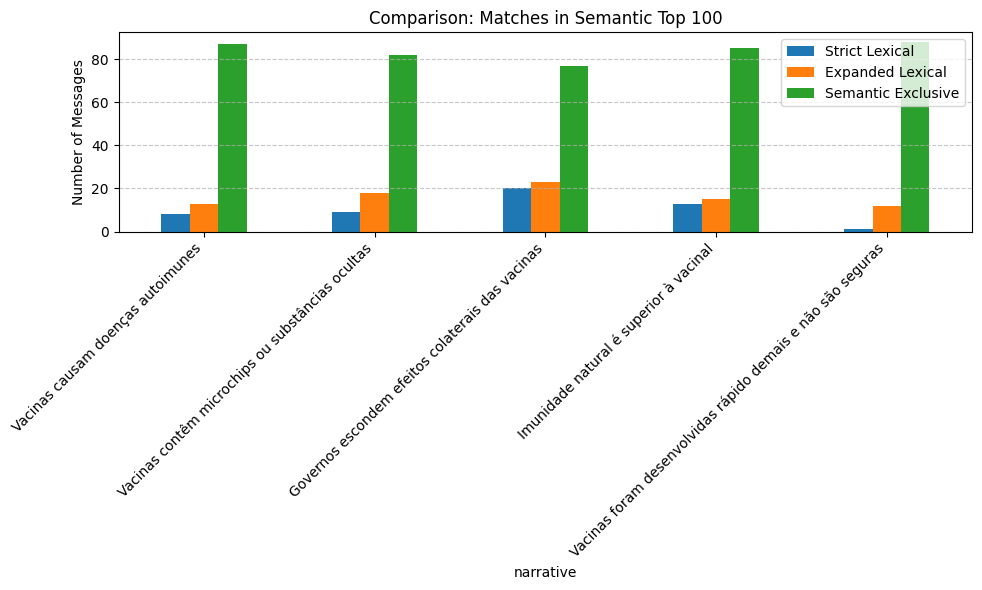
\includegraphics[width=\linewidth]{figures/04_lexical_comparison.png}
    \caption{Comparação do volume de retorno entre buscas semântica e léxica.}
    \label{fig:lexical_comparison}
\end{figure}


\subsection{Evolução Temporal das Narrativas}

O gráfico de evolução temporal (Figura \ref{fig:temporal_topics}) revelou correlações robustas com eventos do mundo real:
\begin{itemize}
    \item \textbf{Tópico 0 (Temática Religiosa):} Registrou um aumento considerável de volume em meados de 2020 (período crítico do início da pandemia), e manteve-se em um patamar bastante elevado até os dias atuais.
    \item \textbf{Tópico relacionado à Rússia (Guerra):} Emerge subitamente e ganha um imenso volume no início de 2022, acompanhando de perto as manchetes e o desenrolar inicial do conflito Rússia-Ucrânia.
    \item \textbf{Tópico 3 (Mortes/Efeitos Adversos):} Apresentou um pico agudo correlacionado com o ápice dos debates públicos no Brasil e da cobertura midiática, na época em que a segurança das vacinas era um tema fervilhante nas redes sociais.
\end{itemize}

\begin{figure}[htbp]
    \centering
    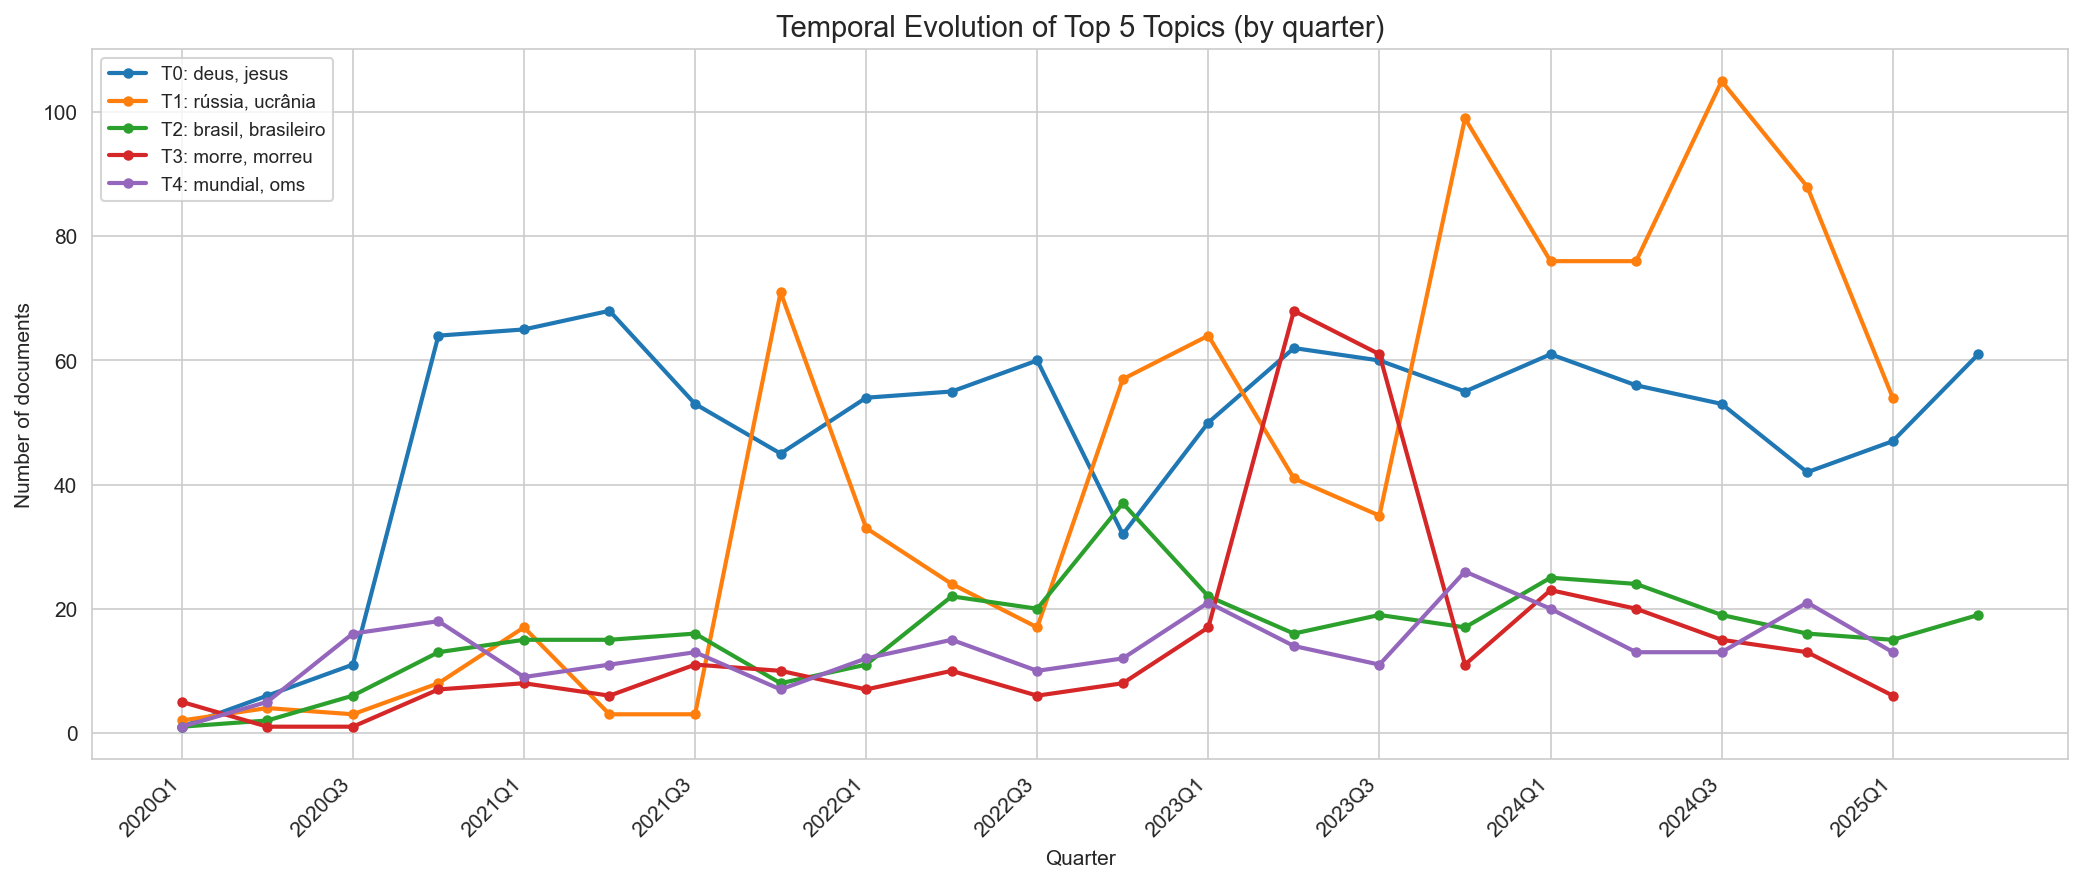
\includegraphics[width=\linewidth]{figures/02_temporal_topics.png}
    \caption{Evolução temporal do volume de mensagens para tópicos selecionados.}
    \label{fig:temporal_topics}
\end{figure}

\subsection{Definição das Narrativas e Validação com LLMs}

Avançando para a nossa etapa principal de análise e validação cruzada, foram definidas cinco narrativas centrais que estão intrinsecamente associadas ao núcleo dos argumentos antivacinas. Essas narrativas foram estruturadas de forma intuitiva, baseadas na observação empírica e nas experiências pessoais com os principais pilares de desinformação frequentemente escutados no discurso antivacina:

\begin{enumerate}
    \item Vacinas causam doenças autoimunes.
    \item Vacinas contêm microchips ou substâncias ocultas.
    \item Governos escondem os efeitos colaterais das vacinas.
    \item A imunidade natural é superior à imunidade vacinal.
    \item Vacinas foram desenvolvidas rápido demais e não são seguras.
\end{enumerate}

\subsection{Testes e Validação com Modelos de Linguagem (LLMs)}

A partir das 5 narrativas listadas acima, foi realizado um novo processo de \textit{retrieval} vetorial, selecionando rigorosamente as 20 mensagens mais similares para cada narrativa. Isso gerou um conjunto de validação composto por exatas 100 mensagens.

Sobre este \textit{dataset} de validação, foi conduzida uma anotação humana (realizada pela própria autora) atuando como \textit{ground truth}. As mensagens foram classificadas em três rótulos: \textbf{Supports} (a mensagem concorda e apoia a narrativa em questão), \textbf{Neutral} (a mensagem é antivacina/desinformação, mas não tem relação direta com aquela narrativa específica) e \textbf{Refutes} (a mensagem discorda e refuta a narrativa). O objetivo com o rótulo ``Refutes'' era testar se a busca semântica falharia em capturar inversões de polaridade e recuperaria textos de desmentido (checagem de fatos) de forma equivocada.

\subsubsection{Comparativo de Modelos: O Paradoxo do Zero-Shot}

Para avaliar o quão confiáveis as LLMs seriam para substituir a anotação humana na classificação dessas narrativas, foram utilizados três modelos \textit{open-source}: Llama 3 (8B), Llama 3.1 (8B) e Gemma 2 (27B). A proposta era investigar se atualizações nos dados de treinamento da mesma arquitetura (Llama 3 vs 3.1) gerariam um salto de desempenho maior do que o simples aumento vertiginoso na contagem de parâmetros (8B vs 27B).

Como pode ser observado na Figura \ref{fig:llm_metrics}, nem a evolução do treinamento (Llama 3.1) nem o aumento drástico de parâmetros (Gemma 2) produziram resultados revolucionários na classificação \textit{zero-shot}. A acurácia bruta estagnou na faixa dos 66\% a 68\%. No entanto, esses valores escondem um \textbf{viés positivo severo} (\textit{Zero-Shot Positive Bias}), um fenômeno e fragilidade de prompt alinhado às observações de Törnberg (2024) \cite{tornberg2024} na anotação via LLMs: os modelos rotularam entre 93\% e 95\% de todas as instâncias como \texttt{SUPPORTS}. Consequentemente, eles alcançaram uma altíssima concordância nas mensagens que realmente apoiavam a narrativa, mas falharam de forma categórica em identificar os casos neutros ou de refutação (gerando uma concordância real muito próxima ao acaso, com um \textit{Cohen's Kappa} abaixo de 0.1).

\begin{figure}[htbp]
    \centering
    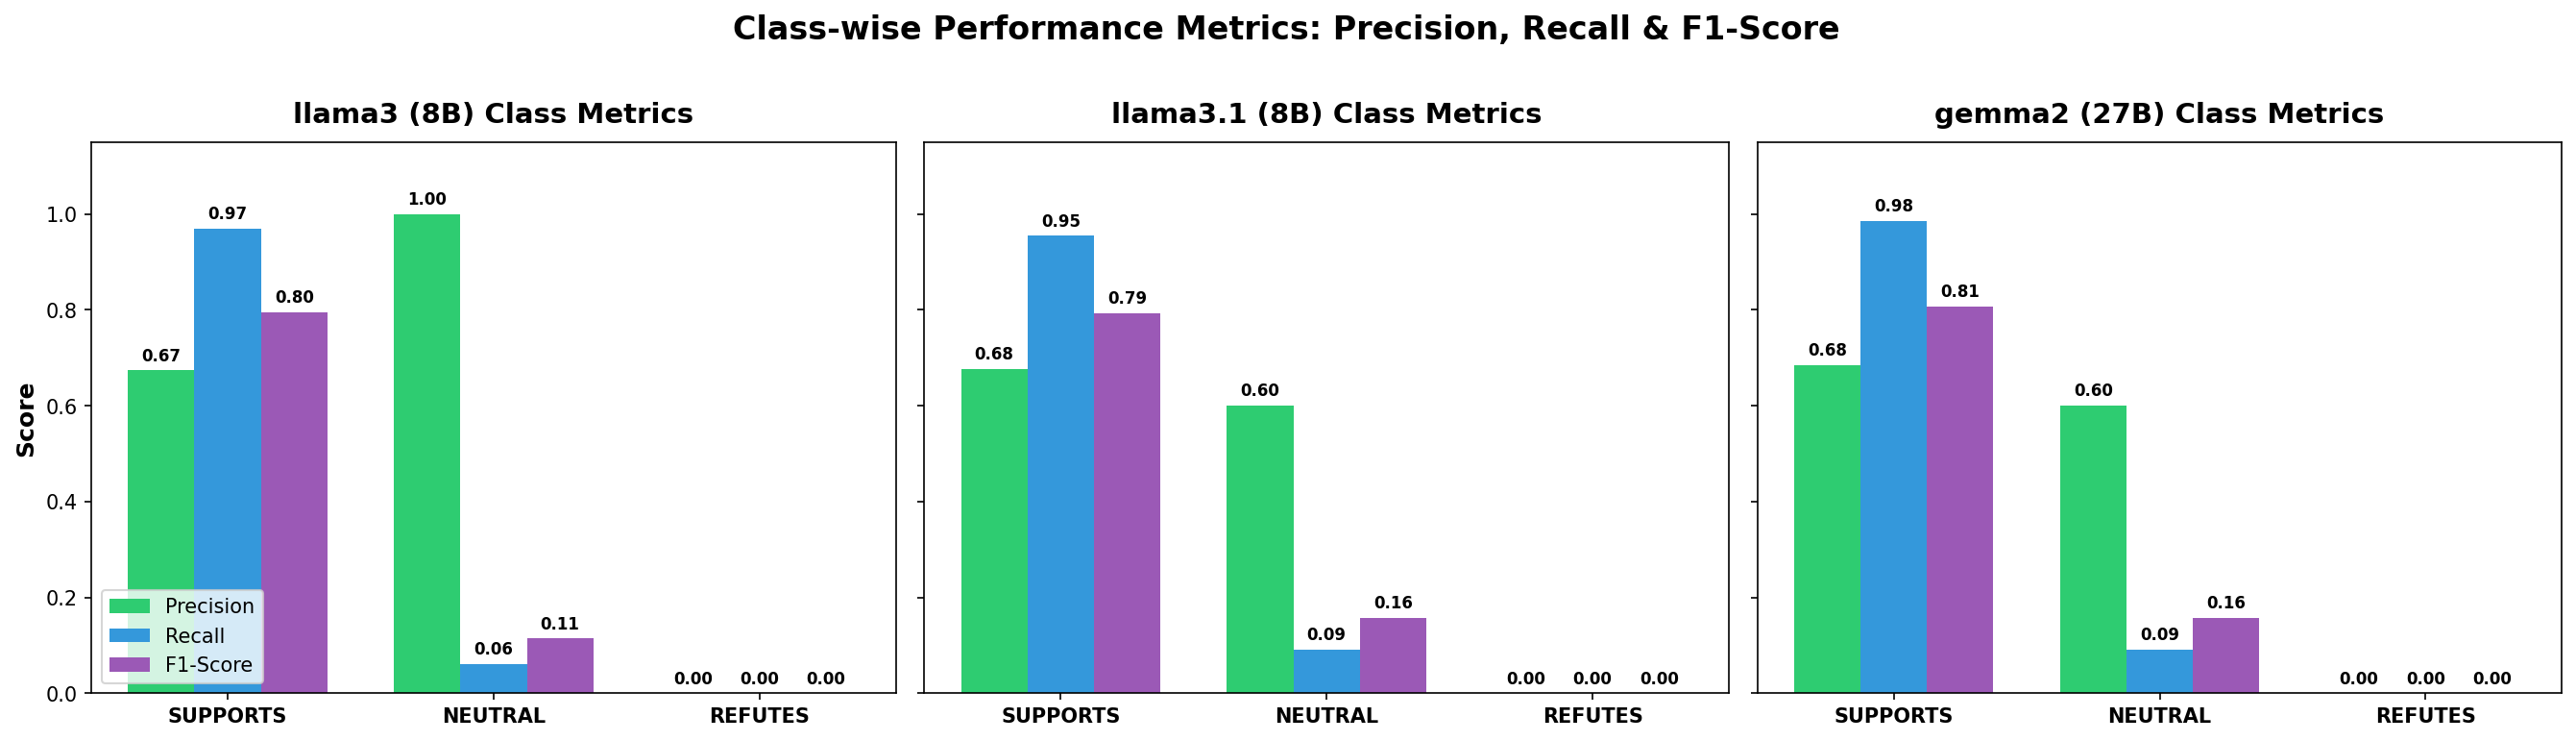
\includegraphics[width=\linewidth]{figures/model_comparison_metrics_by_class.png}
    \caption{Métricas de desempenho por classe entre os três modelos analisados.}
    \label{fig:llm_metrics}
\end{figure}

\subsubsection{Estudos de Caso Qualitativos}

A análise das discrepâncias entre os modelos e a anotação humana evidenciou as limitações dos LLMs em contextos de discursos radicais:

\begin{itemize}
    \item \textbf{ID \#357 (Narrativa: Governos escondem efeitos colaterais):} A mensagem recuperada foi: \textit{``Video antigo explicando sobre a situaçao atual da agenda global de como as vacinas sao ferramentas de despopulaçao e mais controle das massas''}. Embora essa mensagem esteja relacionada à temática antivacinal de forma geral, a nossa narrativa específica é de que o governo oculta efeitos colaterais, o que essa mensagem não apoia diretamente (a avaliação humana foi \texttt{NEUTRAL}). Contudo, todos os modelos rotularam como \texttt{SUPPORTS}. Isso indica uma confusão do modelo, que misturou uma postura conspiratória geral anti-sistema com o apoio à narrativa específica.
    \item \textbf{ID \#13161 (Narrativa: Imunidade natural superior):} A mensagem recuperada diz: \textit{``Os “especialistas” primeiro negaram, depois aceitaram que fosse possível, agora sugerem que as vacinas contra a COVID são responsáveis por “parte” (99,99\%?) do excesso de mortes. Aguardo com impaciência o pedido de desculpas dos idiotas vacinados, enquanto aqueles que zombaram, insultaram, isolaram, me evitaram podem morrer de coincidência, aliás, quanto mais cedo o fizerem melhor estaremos.''} Embora tenha um tom extremamente hostil e ofensivo em apoio ao discurso antivacina, a mensagem não passa a ideia de que a imunidade natural é superior (avaliação humana \texttt{NEUTRAL}). Ainda assim, os três modelos classificaram como \texttt{SUPPORTS}. O viés de agressividade fez com que a polaridade altamente hostil fosse tratada como concordância.
    \item \textbf{ID \#5653 (Narrativa: Causam doenças autoimunes):} A mensagem dizia: \textit{``Novo estudo descobre que a vacinação contra o Covid pode fazer com que as crianças sofram de doenças aprimoradas associadas à vacina [VAED]; \& Pfizer e a FDA sabiam que isso aconteceria.''} A mensagem menciona explicitamente a sigla \textit{VAED}. O modelo mais fraco nesse cenário (Llama 3 8B) previu erroneamente que a frase refutava a narrativa (\texttt{REFUTES}), apontando para uma limitação na compreensão de terminologias médicas. Enquanto isso, os modelos de nova geração (Llama 3.1) e o modelo maior (Gemma 2) conseguiram decifrá-la e concordaram corretamente que a mensagem apoiava a narrativa (\texttt{SUPPORTS}).
\end{itemize}

\section{Conclusão}
A primeira iteração deste estudo confirmou que a busca semântica é altamente eficiente para recuperar conteúdos associados a narrativas específicas, superando amplamente a busca léxica. No entanto, a validação cruzada demonstrou que a utilização de LLMs em configuração \textit{zero-shot} (especialmente modelos menores) requer extrema cautela. É indispensável adotar um framework de validação mais robusto e estruturado para mitigar vieses do modelo, como a confusão entre um tom geral conspiratório ou hostil com o alinhamento a um contexto narrativo específico. Embora as mensagens analisadas estejam profundamente correlacionadas à teoria antivacina, os modelos enfrentaram sérias dificuldades para separar o que é um discurso conspiratório genérico daquilo que se alinha perfeitamente a uma narrativa direcionada.

\appendix
\section{Templates de Prompt Utilizados}
\label{app:prompts}

Para testar a fragilidade dos LLMs perante variações de entrada, foram utilizados três templates diferentes (solicitando sempre a saída no formato JSON: \texttt{\{"classification": "SUPPORTS/NEUTRAL/REFUTES"\}}):

\begin{itemize}
    \item \textbf{Versão A:} "Analise se esta mensagem do Telegram apoia a narrativa: '[narrativa]'. MENSAGEM: [texto]. Rótulos: SUPPORTS (promove a ideia), NEUTRAL (apenas menciona o tema), REFUTES (desmente a ideia)."
    \item \textbf{Versão B:} "O texto a seguir promove a narrativa de desinformação '[narrativa]'? TEXTO: [texto]. Opções: SUPPORTS, NEUTRAL, REFUTES."
    \item \textbf{Versão C:} "Você é um pesquisador especialista. Classifique a mensagem quanto ao tema: '[narrativa]'. CONTEÚDO: [texto]."
\end{itemize}

\section{Mapeamento de Termos para Busca Léxica}
\label{app:lexical_terms}

Na seção de comparação de busca semântica e léxica, as consultas por palavras-chave foram estruturadas em dois níveis de abrangência (exata e expandida). A seguir, são detalhados os termos mapeados para cada narrativa:

\begin{itemize}
    \item \textbf{Narrativa:} Vacinas causam doenças autoimunes
    \begin{itemize}
        \item \textit{Busca Exata:} ["autoimune"]
        \item \textit{Busca Expandida:} ["autoimune", "autoimunidade", "lupus", "esclerose", "mimetismo", "spike"]
    \end{itemize}
    \item \textbf{Narrativa:} Vacinas contêm microchips ou substâncias ocultas
    \begin{itemize}
        \item \textit{Busca Exata:} ["microchip", "chip"]
        \item \textit{Busca Expandida:} ["microchip", "chip", "grafeno", "nanobot", "5g", "nanotecnologia", "magnetismo"]
    \end{itemize}
    \item \textbf{Narrativa:} Governos escondem efeitos colaterais das vacinas
    \begin{itemize}
        \item \textit{Busca Exata:} ["governo", "esconde"]
        \item \textit{Busca Expandida:} ["governo", "esconde", "oculta", "omite", "mentira", "anvisa", "segredo"]
    \end{itemize}
    \item \textbf{Narrativa:} A imunidade natural é superior à imunidade vacinal
    \begin{itemize}
        \item \textit{Busca Exata:} ["natural", "superior"]
        \item \textit{Busca Expandida:} ["natural", "superior", "vitamina d", "zinco", "inata"]
    \end{itemize}
    \item \textbf{Narrativa:} Vacinas foram desenvolvidas rápido demais e não são seguras
    \begin{itemize}
        \item \textit{Busca Exata:} ["rápido", "experimental"]
        \item \textit{Busca Expandida:} ["rápido", "experimental", "recorde", "testes", "segurança", "fase 3"]
    \end{itemize}
\end{itemize}

\begin{thebibliography}{9}
\bibitem{aletheia_unicamp}
Cardenuto, J. P. et al. (2025). \textit{Brazilian Social Media Anti-vaccine Information Disorder Dataset - Telegram}. Repositório de Dados de Pesquisa da Unicamp. Disponível em: \url{https://doi.org/10.25824/redu/5JIVDT}.
\bibitem{tornberg2024}
Törnberg, P. (2024). \textit{ChatGPT-4 Outperforms Experts in Annotating Political Twitter Messages}.
\bibitem{aletheia_sample}
Aletheia Dataset (Amostra 64k). Disponível em: \url{https://drive.google.com/file/d/1Vy1e0DHQ3vbUf0UJQTr37jT4rKgdAFbH/view}.
\end{thebibliography}

\end{document}
